\documentclass[12pt]{article}
\usepackage{fullpage,enumitem,amsmath,amssymb,graphicx,grffile,float,listings}



\begin{document}
    %Title Section
    \begin{flushleft}
    \LARGE CS229 Fall 2017\\
    \LARGE Problem Set \#2:  Supervised Learning II    \\
    \textbf{\normalsize Author: LFhase \quad rimemosa@163.com}
    \end{flushleft} 
    \noindent
    \rule{\linewidth}{0.4pt}
    %Title Section

    %Problem and Solution

    \section*{Logistic Regression: Training stability  }

    \begin{enumerate}[label=(\alph*)]
    \item Training model on dataset A costs far more less time than that on dataset B, which means that training on dataset B does't converge.
    \item 
    Let's plot the training results after 10000, 20000, 30000, 40000 iterations.
    \begin{figure}[H]
        \centering
        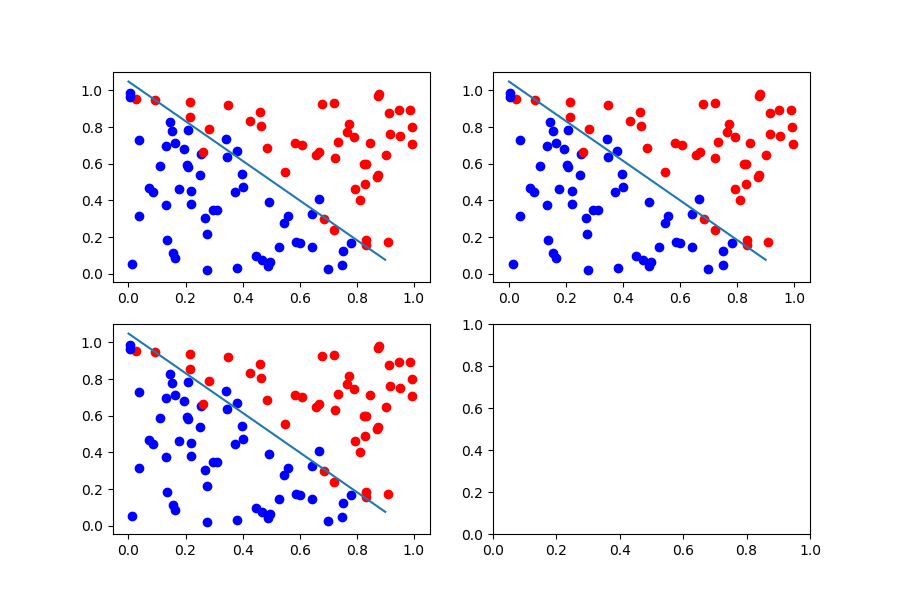
\includegraphics[width=0.80\textwidth]{Q1/training_dsA.png}
        \caption{Training Results on Dataset A}
    \end{figure}
    \begin{figure}[H]
        \centering
        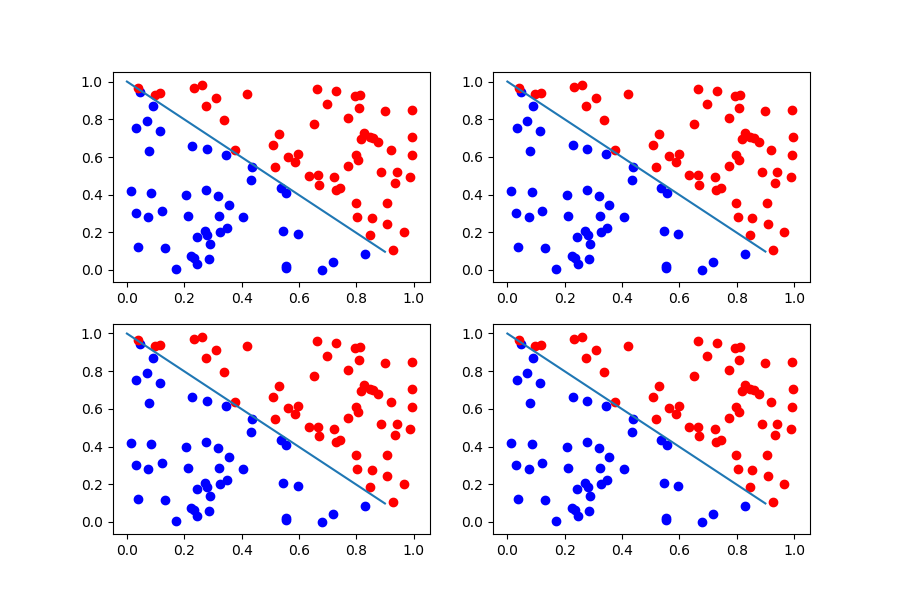
\includegraphics[width=0.80\textwidth]{Q1/training_dsB.png}
        \caption{Training Results on Dataset B}
    \end{figure}
    From the above two figures, we can see that data on dataset B is hardly to separate (Bad Linearly Separability), which may be the main issue resluting nonconvergence.
    \item 
    \begin{enumerate}[label=\roman*]
        \item No. Using a different learning rate only changes the learning speed here, but it won't change the fact that the algorithm has to find the hyperline in hardly separable data.
        \item No. The same to the former.
        \item Yes. It will stop $||\theta||$ being infinitely large.
        \item No. It doesn't change the linearly separability.
        \item Yes. It will expand the feature space, which may let the data linearly separable.
    \end{enumerate}
    \item It's vulnerable. With hinge loss, using slack variables, the formulation will be changed into what's be induced in class.
    \end{enumerate}

    \newpage
    \section*{Model Calibration}
    \begin{enumerate}[label=(\alph*)]
    \item Firstly, we write the log-likelihood function of Logistic Regression:
    $$J(\theta) = \sum_{i=1}^m (y^{(i)}logh(x^{(i)})+(1-y^{(i)})log(1-h(x^{(i)})))$$
    Then, let $$ \frac{\partial J(\theta)}{\partial \theta} = 0 $$ 
    We get $$\sum_{i=1}^m(y^{(i)}-h(x^{(i)}))x^{(i)}_j = 0$$
    Because $x_0 = 1$ for all training examples, so $|X_{m\times n}|\neq 0$ and $y^{(i)}-h(x^{(i)}) = 0$, which means
    $$\sum_{i=1}^mh(x^{(i)}) = \boldsymbol{1}\{y^{(i)}=1\}$$
    The property described in problem statement gets proved.
    \item Perfect calibration means the model has a good performance in training data, which doesn't ensure the model achieves perferct accuray in other conditions.
    However, once a model achieves perferct accuray, it should be perferctly calibrated.
    \item The new log-likelihood function will become
    $$J'(\theta) = J(\theta)+c||\theta||^2 $$
    Let $$ \frac{\partial J'(\theta)}{\partial \theta} = 0 $$ 
    We get $$ \frac{\partial J(\theta)}{\partial \theta} +2c\theta = 0 $$
    which means $$\sum_{i=1}^m(y^{(i)}-h(x^{(i)}))x^{(i)}_j +2c\theta_0= 0$$
    and $$\sum_{i=1}^mh(x^{(i)}) = \boldsymbol{1}\{y^{(i)}=1\}+2c\theta_0$$
    The left part in Model Calibration equation will get $2c\theta_0$ bias.
    \end{enumerate}

    \newpage
    \section*{Bayesian Logistic Regression and weight decay }
    Assume that $||\theta_{MAP}||_2 > ||\theta_{ML}||_2$,
    we can get $$p(\theta_{MAP}) < p(\theta_{ML})$$
    thus $$p(\theta_{MAP})\Pi_{i=1}^{m}p(y^{(i)}|x^{(i)};\theta_{MAP}) < p(\theta_{ML})\Pi_{i=1}^{m}p(y^{(i)}|x^{(i)};\theta_{MAP})$$
    with $$\Pi_{i=1}^{m}p(y^{(i)}|x^{(i)};\theta_{MAP}) < \Pi_{i=1}^{m}p(y^{(i)}|x^{(i)};\theta_{ML})$$
    we get $$p(\theta_{MAP})\Pi_{i=1}^{m}p(y^{(i)}|x^{(i)};\theta_{MAP}) < p(\theta_{ML})\Pi_{i=1}^{m}p(y^{(i)}|x^{(i)};\theta_{ML})$$
    which is contradicted with the definition of $\theta_{MAP}$.

    \section*{Constructing kernels}
    According to Mercer's theorem, if $K(x,z)$ is a kernel, then we have $\mu^T M \mu \geq 0$.
    \begin{enumerate}[label=(\alph*)]
        \item Yes. Since $K_1 \geq 0$ and $K_2 \geq 0$, so $K_1 + K_2 \geq 0$.
        \item No. $K_1 \geq 0$ and $K_2 \geq 0$ doesn't necessarily mean $K_1 - K_2 \geq 0$.
        \item If $a \geq 0$, the answer is 'Yes'. 
        \item If $a \geq 0$, the answer is 'No'.
        \item 
        Since $K_1$ and $K_2$ are valid kernels, we can let $\phi_1$ and $\phi_2$ be their feature map function and $\phi$ be K's.
        Then we have
        \begin{equation*}
            \begin{split}
                K(x,z) &= \phi_1(x)^T\phi_1(z)\phi_2(x)^T\phi_2(z) \\
                &= \sum_{i,j} \phi_1(x)_i\phi_1(z)_i\phi_2(x)_j\phi_2(z)_j \\
                &= \sum_{i,j} [\phi_1(x)_i\phi_2(x)_j][\phi_2(x)_j\phi_1(z)_i]
            \end{split}
        \end{equation*}
        If let $\phi_{i,j} =  {\phi_1}_i{\phi_2}_j $, then we can easily write the inner product formula of $K(x,z)$.
        Through the definition of Kernel, we know that $K(x,z)$ is a valid kernel.
        \item Yes, since $K(x,z) = (\sum_{i=1} \mu_i f(x^{(i)}))^2 \geq 0$.
        \item Yes, since $K(x,z) = \sum_{i,j} \mu_i \mu_j K_3 \geq 0$.
        \item Yes, since $K(x,z) = \sum_{i,j} \mu_i \mu_j (\sum_t a_t {K_1}^t) \geq 0$.
    \end{enumerate}

    \section*{Kernelizing the Perceptron}
    \begin{enumerate}[label=(\alph*)]
        \item gg
    \end{enumerate}
\end{document}